    
\clearpage
\newgeometry{left=-0.50cm,right=-0.50cm,top=0cm,bottom=0cm,centering}
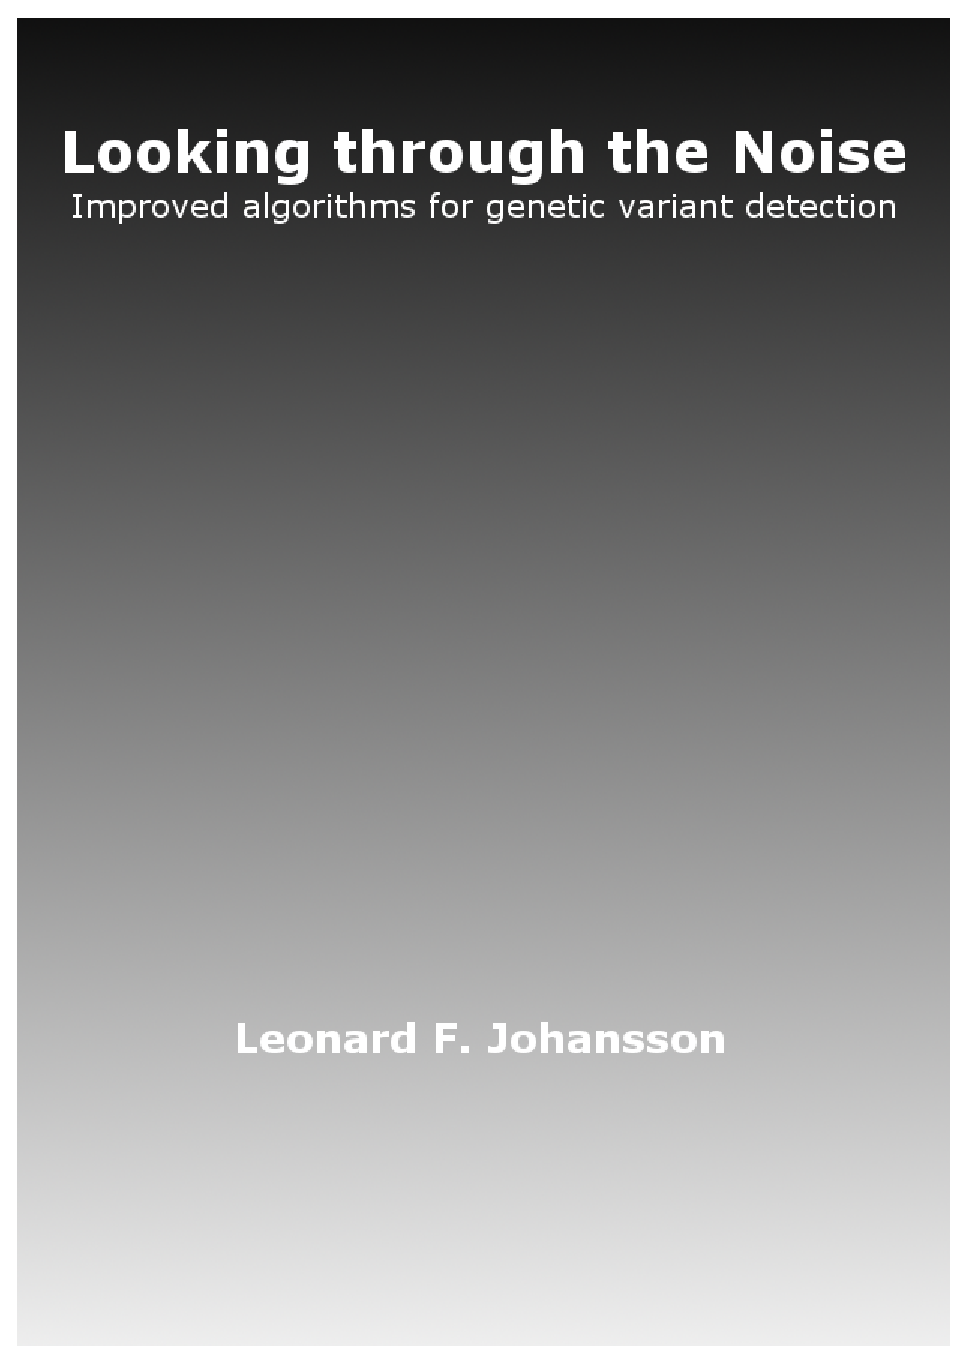
\includegraphics[width=0.935\textwidth,height=1.0\textheight]{img/frontcover_zw}
\restoregeometry
\clearpage

{\small
\noindent
Leonard Fredericus Johansson. \textbf{Looking through the noise: improved algorithms for genetic variant detection.} Thesis, University of Groningen, with summary in English and Dutch.
\\~\\
The research presented in this thesis was mainly performed at the Department of Genetics, University Medical Center Groningen, University of Groningen, Groningen, the Netherlands. Part of the work in this thesis was financially supported by ZONMW, grant no 40-41200-98-9159, Netherlands CardioVascular Research Initiative (CVON2011–19; Genius), and the Netherlands Organization or Scientific Research (NOW) VIDI grant number 917.164.455 received by Morris A. Swertz. 
\\~\\
Printing of this thesis was financially supported by Rijksuniversiteit Groningen, University Medical Center Groningen. 
\\~\\
Cover design and layout by L.F. Johansson.
The front cover shows a variant that can only be seen when looking through the noise created by the four DNA nucleotides A, C, G and T. 
\\~\\
Printed by Ipskamp Drukkers, Enschede.\\
\\
© 2019 L.F. Johansson. All rights reserved. No part of this book may be reproduced or transmitted in any form or by any means without permission of the author.\\
\\
ISBN: XXX-XX-XXX-XXXX-X \mbox{~~~~~} ISBN (electronic version): XXX-XX-XXX-XXXX-X
}

\begin{figure}[!htbp]
  \centering

  \begin{minipage}[b]{0.24\textwidth}
    \includegraphics[width=\textwidth]{img/colofon_umcg_zw}
  \end{minipage}
  \hfill
  \begin{minipage}[b]{0.29\textwidth}
    \raisebox{0.4\height}{\includegraphics[width=\textwidth]{img/colofon_rug_zw}}
  \end{minipage}

\end{figure}

\clearpage

\begin{flushleft}
\includegraphics[scale=0.8]{img/rugr_logonl_zwart_cmyk}
\end{flushleft}

\begin{center}
\linespread{1.00} % squish slightly to fit everyone on page
~\\
\huge
\textbf{Looking through the noise \\ improved algorithms for genetic variation detection}
\\~\\
\linespread{1.05} % and back to normal


\large
\textbf{Proefschrift}
\\~\\
\normalsize
ter verkrijging van de graad van doctor aan de\\
Rijksuniversiteit Groningen\\
op gezag van de\\
rector magnificus prof. dr. E. Sterken\\
en volgens besluit van het College voor Promoties.
\\~\\
De openbare verdediging zal plaatsvinden op
\\~\\
maandag X X 201X om XX.XX uur 
\\~\\~\\
door
\\~\\~\\
\large
\textbf{Leonard Fredericus Johansson}
\\~\\
\normalsize
geboren op 29 mei 1980\\
te Hefshuizen\\
\normalsize
\end{center}

\clearpage

\noindent
\textbf{Promotor}\\
Prof. dr. R.H. Sijmons

\noindent
\textbf{Copromotores}\\
Prof. dr. M.A. Swertz\\
Dr. B. Raddatz

\noindent
\textbf{Beoordelingscommissie}\\
Prof. dr. XX\\
Prof. dr. XX\\
Prof. dr. XX\\


\clearpage

\noindent
\textbf{Paranimfen}\\
E.N. de Boer\\
K.K. van Dijk-Bos\\